\documentclass[main.tex]{subfiles}
\begin{document}


\chapter{Anfänge der Differentialgeometrie}


\section{Implizite Funktionen}

\begin{Beispiel}
  Wir wollen $x^2 = y^3 - y$ 'nach $y$ auflösen', also eine Aussage der Form $y = f(x)$.
  $$F(x,y) = y^3 - y - x^2 \quad F: \R^2 \to \R$$
  Die obige Gleichung zu lösen bedeutet die Nullstellen von $F$ zu finden.
  \begin{center}
    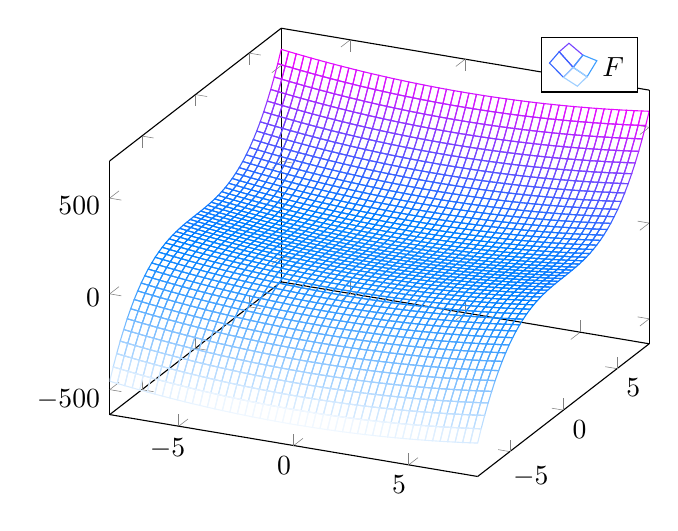
\begin{tikzpicture}
      \begin{axis}[
          % show axis
          colormap/cool,]
      \addplot3[
          mesh,
          samples=50,
          domain=-8:8,]
      {y^3 + y + x^2};
      \addlegendentry{$F$}
      \end{axis}
    \end{tikzpicture}
  \end{center}
  (Man sieht eine in $x$-Richtung angedeutete Parabel)

  Folgendes Problem: die Menge $M = \{(x,y) \mid F(x,y) = 0\}$ definiert keinen Funktionsgraphen.
\end{Beispiel}

Allgemein betrachten wir $F : U \subseteq \R^n \times \R^m \to \R^m$. Wir behalten aber die Notation $F(x,y) = 0$, wobei $x$ und $y$ Vektoren sind, und die Null ebenfalls.

Dies aufzulösen entspricht eienem System von $m$ Gleichungen in $n+m$ Variablen (und wir wollen nach $n$ Komponenten auflösen).

\begin{Theorem}[Satz der impliziten Funktion]
  Sei $U \subseteq \R^n$ offen, $(x_0,y_0) \in U$ und $F: U \to \R^n$ stetig mit folgenden Hypothesen:
  \begin{enumerate}
    \item $F(x_0,y_0) = 0$
    \item Die partiellen Ableitungen $\frac{\partial}{\partial y_k} F : U \to \R^m$ existieren und sind stetig.
    \item Die Matrix
      $$A = \left(\dfrac{\partial}{\partial y_k} F_j (x_0,y_0)\right)_{k,j} \in M(m,\R)$$
      ist invertierbar.
  \end{enumerate}
  Dann existieren $r > 0$, $s > 0$ und eine stetige Funktion $f: B(x_0, r) \to B(y_0,s)$ so, dass
  $$\A (x,y) \in B(x_0, r) \times B(y_0,s) : F(x,y) = 0 \Leftrightarrow y = f(x)$$
  Angenommen $F \in \mathcal{C}^d$, $d \geq 1$, dann ist $f \in \mathcal{C}^d$ und es gilt:
  $$Df(x) = -(D_y F(x,f(x)))^{-1} \circ (D_x F(x,f(x)))$$
\end{Theorem}

\begin{Bemerkung}
  Hier bedeutet $D_x F(x_1,y_1)$: die totale Ableitung der Funktion $x \mapsto F(x,y_1)$ am Punkt $x_1$ (analog für $D_y F$).
\end{Bemerkung}

\begin{Bemerkung}
  Testen wir, ob diese Formel sinnvoll ist:
  $$Df(x) : \R^n \to \R^m$$
  $$D_y F(x,f(x)) : \R^m \to \R^m \quad D_x F(x,f(x)): \R^n \to \R^m$$
\end{Bemerkung}

\begin{Beweis}
  OBdA gilt $U = B_N \times B_m$ mit $B_n = B(x_0,r_0)$ und $B_m = B(y_0,s_0)$. Für ein fixes $x \in B_n$ schreibe
  $$B(x_0, r) \to B(y_0,s) \quad F_x(y) = F(x,y)$$
  Die Matrix $A$ ist die Jacobi-Matrix von $F_{x_0}$ im Punkt $y_0$ entsprechend $DF_{x_0}(y_0)$. Weiter definieren wir für das fixe $x \in B_n$ die Hilfsfunktion
  $$T_x: B_m \to \R^m \quad T_x(y) = y - A^{-1} \cdot F_x(y)$$
  Bemerke $F(x,y) = 0 (\Leftrightarrow A^{-1} \cdot F_x(y) = 0) \Leftrightarrow T_x(y) = y$

  \begin{Theorem}
    $\E r>0, s>0 : \A x \in B(x_0,r)$ sich die Funktion $T_x$ zu einer Lipschitz-Kontraktion $T_x : \overline{B(y0,r)} \to \overline{B(y_0,r)}$ einschränkt.
  \end{Theorem}
  \begin{Beweis}
    Die Abbildung $B_n \times B_m \to Hom(\R^m,\R^m)$ (versehen mit Operator-Norm ist er sogar eine metrischer Raum), gegeben durch $x,y \mapsto DT_x(y)$ ist stetig.

    Für $x_0,y_0$ gilt
    $$DT_{x_0}(y_0) = id_m - A^{-1} \cdot A = 0$$
    Es existieren also $r > 0, s>0$ mit
    $$\begin{array}{c}
      x \in B(x_0,r) \\ y \in B(y_0,s)
    \end{array}
    \Rightarrow ||DT_x(y)|| \leq \dfrac{1}{2}$$
    Für $x \in B(x_0,r)$, $y_1,y_2 \in B(y_0,s)$ setze $\gamma(t) = (1-t)y_1 + ty_2$.

    Rechne
    $$\begin{aligned}
      ||T_x(y_1) - T_x(y_2)|| & = ||(T_x \circ \gamma)(1) - (T_x \circ \gamma)(0)|| \\
      & = \left|\left|\int_0^1 (T_x \circ \gamma)'(t)dt\right|\right| \\
      & \stackrel{dg}{\leq} \int_0^1 ||D T_x(\gamma(t))(y_2 - y_1) || dt \\
      & \leq \int_0^1 \underbrace{||D T_x(\gamma(t))||_{op}}_{\leq \frac{1}{2}} \cdot ||y_2 - y_1|| dt \\
      & \leq \dfrac{1}{2} \cdot ||y_2 - y_1||
    \end{aligned}$$
    Ist das Bilt von $T_X : \overline{B(y_0,r)} \to \R^m$ in $\overline{B(y_0,r)}$ enthalten?

    $F$ ist stetig und $F(x_0,y_0) = 0$,also $T_{x_0}(y_0) = y_0$. Für $x \in B(x_0,r)$ mit $r>0$ klein genug gilt
    $$||T_x(y_0) - y_0|| \leq \dfrac{s}{2}$$
    Folgt:
    $$\begin{aligned}
      ||T_x(y) - y_0|| & = ||T_x(y) - T_x(y_0) + T_x(y_0) -y_0|| \\
      & \leq \underbrace{||T_x(y) - T_x(y_0)||}_{\leq \frac{1}{2}s} + \underbrace{|| T_x(y_0) -y_0||}_{\leq \frac{1}{2}} \\
      & \leq s
    \end{aligned}$$
  \end{Beweis}
  Der Ball $\overline{B(y_0,s)}$ ist beschränkt, abgeschlossen also kompakt also vollständig. Folgt dank Banach'schem Fixpunktsatz:
  $$\A x \in \overline{B(x_0,r)} \E! y \in \overline{B(y_0,s)} : T_x(y) = y$$
  Setze $f:\overline{B(x_0,r)} \to \overline{B(y_0,s)} \quad f(x) = y$.

  Stetigkeit von $f$: (ebenfalls Banach.)

  $$\Omega := \{g : \overline{B(x_0,r)} \to \overline{B(y_0,s)} \mid g \text{ ist stetig}\}$$
  $$||g_1 - g_2||_\infty = \max\{|g_1(x) - g_2(x)| \mid x \in \overline{B(x_0,r)}\}$$
  Dieser Raum ist \textbf{vollständig}.
  $$\begin{array}{c c c}
    \tilde{T}: \Omega & \to & \Omega \\
    \tilde{T}(g)(x) & = & g(x) - A^{-1} \cdot F(x,g(x)) \quad \in \overline{B(y_0,s)}
  \end{array}$$
  Für $g_1,g_2 \in \Omega$ gilt
  $$||\tilde{T}(g_1) - \tilde{T}(g_2)||_\infty = \max ||\tilde{T}(g_1) - \tilde{T}(g_2)|| \leq \dfrac{1}{2} ||g_1(x) - g_2(x)|| = \dfrac{1}{2} ||g_1 - g_2||$$
  $$\Rightarrow \tilde{T} \text{ ist eine Lipschitz-Kontraktion}$$
  Sei $\tilde{f}$ der eindeutige Fixpunkt von $\tilde{T}$:
  $$\tilde{T}\tilde{f} = \tilde{f} \Rightarrow T_x(\tilde{f}(x)) = \tilde{f}(x) \A x$$
  Also ist $f = \tilde{f}$ $\Rightarrow f$ ist stetig.
\end{Beweis}

\begin{Beweis}[Wohldefiniertheit der Gleichung $D F$]
  Nach Annahme ist $A = D_y F(x_0,y_0) = D_y F(x_0,f(x_0))$ invertierbar.

  Die Funktion $x \mapsto det(D_y F(x,f(x)))$ ist stetig. Außerdem gilt $x_0 \mapsto det(A) \neq 0$.

  Folgt, dass $D_y F(x,f(x))$ invertierbar ist, für $x \in B(x_0,r)$ für $r$ klein genug.

  Dieses kleine $r$ können wir für verschiedene $x_0$ betrachten und so insgesamt einen Ball mit dem größeren $r$ aus der Aussage konstruieren.
\end{Beweis}

\begin{Beweis}[Gleichheit für $d = 1$]
  \textbf{Notation}:
  \begin{itemize}
    \item $x \in B(x_0,r)$ fix
    \item $A_x = D_y F(x,f(x))$ (also $A_{x_0} = A$)
    \item $a = ||A_x^{-1}||_{op}$
    \item $L_x = -A_x^{-1} \cdot D_x F(x,f(x))$ (rechte Seite der zu beweisenden Formel)
    \item $b = ||L_x||_{op}$
  \end{itemize}
  Für $h \in \R^n$ klein genug so, dass $x + h \in B(x_0,r)$ erhalten wir
  $$\begin{aligned}
    ||f(x+h) - f(x) - L_x(h)|| & \stackrel{\scriptscriptstyle ZZ}{\leq} \alpha(h) \cdot ||h|| \text{ mit } \alpha(h) = o(1) \\
    & \leq ||f(x+h) - f(x) + A_x^{-1}\cdot D_x F(x,f(x)) \cdot h|| \\
    & \leq a \cdot ||D_x F(x,f(x))(h) + \underbrace{D_y F(x,f(x))}_{A_x}(f(x+h) -f(x))|| \\
    & = a \cdot ||DF(x,f(x))(h,f(x)+h - f(x))|| \\
    & = a \cdot ||\underbrace{F(x+h,f(x+h))}_{0} \\
    & - \qquad \qquad \underbrace{F(x,f(x))}_{0} - DF(x,f(x))(h,f(x)+h - f(x))|| \\
    & \leq \alpha(h) \cdot ||(h,f(x+h)-f(x))|| \\
    & \text{ mit } \alpha(h) = o(1) \text{ also } \alpha \to 0 \text{ (für } h \to 0)
  \end{aligned}$$
  ZZ: $||f(x+h) - f(x)|| \leq c \cdot ||h|| \Leftrightarrow \alpha(h)(1+c) \cdot ||h||$.

  Nebenrechnung:
  $$\begin{aligned}
    ||f(x + h) - f(x)|| & \leq ||f(x+h) - f(x) -L_x(h) + L_x(h)|| \\
    & \leq ||f(x+h) - f(x) -L_x(h)|| + ||L_x(h)|| \\
    & \leq \alpha(h)(||h|| + ||f(x+h)-f(x)||) + b \cdot ||h||
  \end{aligned}$$

  Wählt man $h$ klein genug, gilt: $\alpha(h) < \frac{1}{2}$.
  $$(1 - \alpha(h)) \cdot ||f(x+h) - f(x)|| \leq (\alpha(h) + b) \cdot ||h|| \Leftrightarrow ||f(x + h) - f(x)|| \leq \underbrace{2 \left(\dfrac{1}{2} + b\right)}_{c} \cdot ||h|$$
  Es folgt die gewünschte Abschätzung.
\end{Beweis}

\begin{Beweis}[für $d \geq 1$ (Induktion)]
  Ist $F$ von Klasse $\mathcal{C}^2$, gilt
  $$Df(x) = - (D_y F(x,f(x)))^{-1} \circ (D_x F(x,f(x)))$$
  Zu zeigen: $Df(x) \in \mathcal{C}^1$ also die Jakobi-Matrix hat Einträge in $\mathcal{C}^1$.
  \begin{itemize}
    \item $D_x F(x,y)$ ist eine Matrix mit Einträgen von Klasse $\mathcal{C}^1$
    \item $D_x F(x,f(x))$ ist eine Matrix mit Einträgen von Klasse $\mathcal{C}^1$
    \item $D_y F(x,f(x))$ ist eine Matrix mit Einträgen von Klasse $\mathcal{C}^1$
  \end{itemize}
  Folgt, dass $D f(x)$ eine Matrix mit Einträgen aus $\mathcal{C}^1$ ist. $\Rightarrow f \in \mathcal{C}^2$.

  Analog: ist $F$ von Klasse $\mathcal{C}^d$, so gilt:

  ... $\Rightarrow Df(x)$ hat Einträge der Klasse $\mathcal{C}^{d-1}$ $\Rightarrow f \in \mathcal{C}^d$
\end{Beweis}

\begin{Beispiel}
  $$U = \R^3 \times \R^2 \sim (\underbrace{x_1,x_2,x_3}_{x},\underbrace{y_1,y_2}_{y})\quad m = 2, n = 3$$
  $$F(x,y) = \left(\begin{array}{c}
    x_1 + x_2^2 + x_3^3 + y_1 + y_2^2 + x_1 y_1 \\
    x_1 + x_2 + \sin(x_3) + 7 \sin(y_2)
  \end{array}\right)
  = \left(\begin{array}{c}
    F_1(x,y) \\
    F_2(x,y)
  \end{array}\right)$$
  Setze $(x_0,y_0) = (0,0)$.

  Also gilt:
  $$D_y F (x,y) = \left(\dfrac{\partial}{\partial y} F_i (x,y)\right)
  = \left(\begin{array}{c c}
    1 + x_1 & 2y_2\\
    0 & 7 \cos(y_2)
  \end{array}\right)$$

  $$A := D_y F(x_0,y_0) = \left(\begin{array}{c c}
    1 & 0 \\
    0 & 7
  \end{array}\right) \quad
  A^{-1} = \left(\begin{array}{c c}
    1 & 0 \\
    0 & \frac{1}{7}
  \end{array}\right)$$

  $$D_x F (x,y) = \left(\dfrac{\partial}{\partial y} F_i (x,y)\right)
  = \left(\begin{array}{c c c}
    1 + y_1 & 2x_2 & 3 x_3^2 \\
    1 & 1 & \cos(x_3)
  \end{array}\right)$$
  $$B := D_x F(x,y) = \left(\begin{array}{c c c}
    1& 0 & 0 \\
    1 & 1 & 1
  \end{array}\right)$$
  $$\begin{aligned}
    f: B(0,r) & \to \R^2 \\
    (x_1,x_2,x_3) & \mapsto (f_1(x_1,x_2,x_3),f_2(x_1,x_2,x_3)) \\
    f(0) & = 0
  \end{aligned}$$

  $$Df(0) = -(DyF(x_0,f(x_0)))^{-1} \circ D_x F(x_0,f(x_0)) = A^{-1} \cdot B = - \left(\begin{array}{c c c}
    1 & 0 & 0 \\
    \frac{1}{7} & \frac{1}{7} & \frac{1}{7}
  \end{array}\right)$$
  \textbf{Explizite Berechnung von $f$} (idR nicht möglich)

  $$y_2 = \sin^{-1}\left(\dfrac{1}{7} (-x_1 - x_2 - \sin(x_3)\right)$$
  also
  $$y_1 = - \dfrac{1}{1 + x_1} \cdot (-x_1 - x_2^2 - x_3^3 - \sin^{-1}(...)^2)$$
  Also:
  $$\left(\begin{array}{c}
    y_1 \\ y_2
  \end{array}\right) = f(x_1,x_2,x_3)$$
  Jetzt gilt
  $$Df(0) = \left(\begin{array}{c c c}
    -1 & 0 & 0 \\
    -\frac{1}{7} & -\frac{1}{7} & -\frac{1}{7}
  \end{array}\right)$$
\end{Beispiel}

\begin{Theorem}[Satz der inversen Funktion]
  Sei $U \subseteq \R^n$ offen und sei $f: U \to \R^n$ von Klasse $\mathcal{C}^d$ mit $d \geq 1$. Sei $x_0 \in U$ mit $Df(x_0)$ invertierbar. Dann existieren offene Umgebungen $U_0$ von $x_0$ und $V_0$ von $y_0 := f(x_0)$ so, dass sich $f$ zu einer Bijektion
  $$f |_{U_0} : U_0 \to V_0$$
  einschränkt.

  Die zu $f |_{U_0}$ inverse Funktion $g: V_0 \to U_0$ ist von Klasse $\mathcal{C}^d$ und es gilt:
  $$Dg(y) = (Df(x))^{-1} \A x \in U \text{ und } y = f(x)$$
  (alternativ $\A y \in V_0 \text{ und } x =g(y)$)
\end{Theorem}

\begin{Beweis}
  Betrachte $F: U \times \R^n \to \R^n$ gegeben durch
  $$F(\underbrace{x}_{\in U}, \underbrace{y}_{\in \R^n}) = f(x) -y$$
  Wir wollen nach $x$ auflösen. Da
  $$D_x F (x_0,y_0) = Df(x_0)$$
  invertierbar ist, können wir den Satz der impliziten Funktion anwenden. Es existieren also $r > 0, s >0$ und $g: B(y_0,r) \to B(x_0,s)$ mit $y(y_0) = x_0$ und
  $$F(x,y) = 0 \Leftrightarrow x = g(y) \A x,y \in B(x_0,s) \times B(y_0,r)$$
  Setze $V_0 = B(y_0,r)$ und $U_0 = g(V_0) = f^{-1}(v_0)$ (also offen mit $x_0 \in U_0$).

  Außerdem gilt (immer noch laut dem Satz der impliziten Funktion), dass $g \in \mathcal{C}^d$ und dass
  $$Dg(y) = -(Dx F(g(y),y))^{-1} \circ D_y F(g(y),y)$$
  Setze nun $g(y) = x$ und $y = f(x)$. Dann gilt
  \begin{itemize}
    \item $(Dx F(g(y),y))^{-1} = Df(x)^{-1}$
    \item $D_y F(g(y),y) = - id$
  \end{itemize}
  Also ist
  $$Dg(y) = Df(x)^{-1}$$
\end{Beweis}

\begin{Beispiel}['Kugelkoordinaten']
  $$\begin{aligned}
    f: \R^3 & \to \R^3 \\
    (r,\vartheta, \varphi) & \mapsto \left(\begin{array}{c}
      r \sin(\vartheta) \cos(\varphi) \\
      r \sin(\vartheta) \sin(\varphi) \\
      r \cos(\vartheta)
    \end{array}\right)
  \end{aligned}$$
  Berechnen wir:
  $$\begin{aligned}
    Df(r, \vartheta, \vartheta) & =\left(\begin{array}{c c c}
      | & | & | \\
      \partial_r f & \partial_\vartheta f & \partial_\varphi \\
      | & | & |
    \end{array}\right)\\
    & = \left(\begin{array}{c c c}
      \sin(\vartheta) \cos(\varphi) & r \cos(\vartheta) \cos(\varphi) & -r \sin(\vartheta) \sin(\varphi)\\
      \sin(\vartheta) \sin(\varphi) & r \cos(\vartheta) \sin(\varphi) & r \sin(\vartheta)\cos(\varphi)\\
      \cos(\vartheta) & -r \sin(\vartheta) & 0
    \end{array}\right)
  \end{aligned}$$
  Ist diese Abbildung invertierbar?
  $$det(Df(r, \vartheta, \varphi)) = r \sin(\vartheta)$$
  Also ist $Df$ invertierbar bei $r \neq 0$ und $\vartheta \neq k \cdot \pi$
\end{Beispiel}

\begin{Beispiel}
  Wir betrachten
  $$\begin{aligned}
    F : \R^2 & \to \R^2 \\
    F(x,y) & = x^2 + y^3 - y
  \end{aligned}$$
  Nullstellen von $F$:
  Bild, hehe:
  Wir wählen als Beispiel: $y_0 = 0.75$ also $y_0 - y_0^3 = \frac{21}{64}$ und $x_0 = \sqrt{\frac{21}{64}}$
  $$\begin{aligned}
    D_y F(x_0,y_0) & = 3 y_0^2 - 1 \in \R \\
    & = \frac{3 \cdot 3^2}{4^2} - 1 = \dfrac{11}{16} \neq 0
  \end{aligned}$$
  Es existiert $f: B(x_0,r) \to B(y_0,s)$ mit $f(x_0) = y_0$ und $F(x,y) = \Leftrightarrow y = f(x)$.
  $$\begin{aligned}
    Df(x_0)(1) := f'(x_0) & = -(D_yF(x_0,y_0))^{-1} \circ D_x F(x_0,y_0) \\
    & = - \dfrac{16}{11} \cdot 2 \sqrt{\dfrac{21}{64}} \\
    & = \dfrac{-32 \sqrt{21}}{88}
  \end{aligned}$$
\end{Beispiel}

\begin{Beispiel}
  Eher ein Gegenbeispiel:
  $$\begin{aligned}
    f: \R & \to \R \\
    f(x) & = x^3
  \end{aligned}$$
  ist bijektiv und von Klasse $\mathcal{C}^\infty$ aber ihr Inverses $g(y) = \sqrt[3]{y}$ ist nicht einmal von Klasse $\mathcal{C}^1$
\end{Beispiel}

\begin{Definition}[Diffeomorphismen]
  Seien $U,V \subseteq \R^n$ offen. Eine Abbildung $f: U \to v$ heißt \textbf{Diffeomorphismus} falls
  \begin{itemize}
    \item $f$ bijektiv ist
    \item $f$ von Klasse $\mathcal{C}^1$ ist
    \item ihr Inverses auch von Klasse $\mathcal{C}^1$ ist
  \end{itemize}
\end{Definition}

\begin{Beispiel}
  $$\begin{aligned}
    f : \R^2 \backslash\{0\} & \to \R^2 \backslash\{0\} \\
    f(x_1,x_2) & = \left(\begin{array}{c}
      x_1^2 - x_2^2 \\ x_1 x_2
    \end{array}\right)
  \end{aligned}$$
  Ist surjektiv. Es gilt
  $$det(Df(x_1,_2)) = 2(x_1^2 + x_2^2) \neq 0$$
  Allerding ist $f$ nicht injektiv: $f(x_1,x_2) = f(-x_1,-x_2)$
\end{Beispiel}

\begin{Theorem}[Satz von Hadamard-Caccioppoli]
  Sei $U \subseteq \R^n$ offen, $f: U \to \R^n$ von Klasse $\mathcal{C}^d$ und injektiv. Angenommen $Df(x)$ sei für jeden Punkt $x \in U$ invertierbar. Dann ist $V= f(U) \subseteq \R^n$ offen und $f$ ein $\mathcal{C}^d$-Diffeomorphismus mit
  $$(Df^{-1})(y) = (Df(x))^{-1}$$
  für alle $x \in U$ und $y = f(x) \in V$.
\end{Theorem}

\begin{Bemerkung}
  Diese Aussage ist eigentlich sogar ein Korollar zum Satz der inversen Funktion. Die Aussage zur Inversen der Ableitung ist dabei äquivalent formuliert.
\end{Bemerkung}

\begin{Beweis}
  Zuerst zeigen wir, dass $V = f(U)$ offen ist. Sei für $x_0 \in U$ $y_0 = f(x_0)$. Da $Df(x_0)$ invertierbar ist, wenden wir den Satz der inversen Funktion an und bekommen offene Umgebungen $U_0$ von $x_0$ und $V_0$ von $y_0$ so, dass $f|_{U_0} : U_0 \to V_0$ ein $\mathcal{C}^d$-Diffeomorphismus ist.

  Insbesondere ist $V_0 = f(U_0) \subseteq f(U) = V$ und also $V$ offen, da $x_0$ und somit $y_0 \in V$ beliebig waren.

  Des Weiteren haben wir
  $$(f|_{U_0})^{-1}: V_0 \to U_0 \Leftrightarrow f^{-1}|_{V_0}: V_0 \to U_0$$
  ($f^{-1}: V \to U$ existiert wegen der Voraussetzung der Injektivität.) Also ist $f^{-1}|_{V_0}$ auch in $\mathcal{C}^d$. Da $y_0$ beliebig war und die stetige Differenzierbarkeit lokal gilt, gilt nun allgemein: $f^{-1} \in \mathcal{C}^d$. Also ist $f: U \to V$ ein $\mathcal{C}^d$-Diffeomorphismus.
\end{Beweis}


\section{Teilmannigfaltigkeiten des $\R^n$}

Wir betrachten den 'euklidischen $\R^n$', also $\R^n$ zusammen mit dem Standardskalarprodukt und also auch einer Norm und einer Metrik.

\begin{Bemerkung}
  \textbf{Mannigfaltigkeiten - Meta}:

  ($\sim$ Kurve oder Fläche im $\R^n$, zum Beispiel eine Kugeloberfläche)

  Höherdimensional: Begriff der Varietät.
\end{Bemerkung}

\begin{Bemerkung}[Voraussetzung]
  Nachfolgend sind alle Funktkionen und Diffeomorphismen, die wir behandeln immer implizit von Klasse $\mathcal{C}^\infty$
\end{Bemerkung}

\begin{Definition}[Mannigfaltigkeit]
  Seien $a \leq k \leq n$ und sei $M \subseteq \R^n$. Wir sagen $M$ sei ein $k$-dimensionale \textbf{Mannigfaltigkeit} falls zu jedem Punkt $p \in M$ eine offene Umgebung $U_p$ von $p \in \R^n$ und ein Diffeomorphismus
  $$\varphi_p : U_p \to V_p \subseteq \R^n$$
  existiert, mit der Eigenschaft
  $$\varphi^{-1} (V_p \cap \R^k \times \{0\}^{n-k}) = U_p \cap M$$
  $$(\Leftrightarrow \varphi(U_p \cap M) = V_p \cap \R^{k} \times \{0\}^{n-k})$$
  \incfig{mannigfaltigkeit}
  $$\R^2 \quad n = 2 \quad k = 1$$
  Wir nennen
  \begin{itemize}
    \item $\varphi_p: U_p \to V_p$ eine Karte (um $p$)
    \item $\varphi^{-1}: V_p \to U_p$ eine Parametrisierung (um $p$)
  \end{itemize}
  Eine Familie von Karten $(U_i, V_i, \varphi_i)_{i \in \mathcal{I}}$ nennen wir \textbf{Atlas} falls jeder Punkt von $M$ im Definitionsbereich einer Karte liegt.
\end{Definition}

\begin{Beispiel}
  $$\underbrace{\R^k \times \{0\}}_{M} \subseteq \R^n$$
  ist eine $k$-dimensionale Teilmannigfaltigkeit.

  Allgemeiner:
  \begin{Theorem}
    Jeder $k$-dimensionaler linearer Untervektorraum von $\R^n$ ist eine $k$-dimensionale Teilmannigfaltigkeit.
  \end{Theorem}
\end{Beispiel}

\begin{Beispiel}[Graphen von glatten Funktionen (wichtig)]
  Sei $n = k +m$, sei $U \subseteq \R^k$ offen und sei $f:U\to \R^m$ glatt.
  $$M = Graph(f) = \{(x,f(x)) \mid x \in U \} \subseteq U \times \R^m \subseteq \R^k \times \R^m (= \R^n)$$
  ist eine Teilmannigfaltigkeit von $\R^n$.

  \textbf{Karte:}
  $$\begin{aligned}
    \varphi : U \times \R^m & \to U \times \R^m \\
    (x,y) & \mapsto (x,f(x)-y)
  \end{aligned}$$
  $$\varphi^{-1}(x,y) = (x,-f(x)-y)$$
  weil $\varphi^{-1}(\varphi(x,y)) = \varphi^{-1}(x,f(x)-y) = (x,f(x)-(f(x)-y)) = (x,y)$
  Also ist $\varphi$ ein Diffeomorphismus und $M$ ist eine Teilmannigfaltigkeit. (Sonderfall weil nur von einer einzigen Karte abgedeckt.)
\end{Beispiel}

\begin{Beispiel}[Einheitssphäre]
  $$M := \left \{ (x_0,x_1,...,x_n) \in \R^{n+1} \Big | \sum \limits_{i=0}^n x_i^2 (= ||x||) = 1 \right \} = \mathbb{S}^n$$
  Für $p \neq e_n$ können wir folgende Karte konstruieren:
  $$U_p \subseteq \R^{n+1} \quad U_p = \{(x_0,...,x_n) \mid x_n < 1\} \quad V_p ) U_p$$
  \incfig{einheitssphaere}
  zu jedem $x \in U$ existiert genau eine Gerade durch $e_n$ und $x$. Schreibe $E(x)$ für den eindeutigen Schnittpunkt mit der Ebene $x_n = 0$ und $Q(x)$ für den Schnittpunkt mit $\mathbb{S}^n = M$.

  Setze $\varphi(x) = (x - e_n) \cdot \dfrac{||E(x) - e_n||}{||Q(x)-e_n||} + e_n$ (stereographische Projektion)
\end{Beispiel}

\begin{Beispiel}
  $$M = \{x,y \mid x^2 + y^3 - y = 0\}$$
  Definiert eine Teilmannigfaltigkeit, die bis auf Variablenvertauschung auch auf kleinen Umgebungen einen Funktionsgraphen beschreibt.
\end{Beispiel}

Dies Motiviert Folgendes:

\begin{Theorem}
  Eine Teilmenge $M \subseteq \R^n$ ist genau dann eine $k$-dimensionale Teilmannigfaltigkeit, wenn zu jedem Punkt $p \in M$ eine offene Umgebung $U_p$ von $p$ in $\R^n$, eine glatte Funktion $f_p: \tilde{U}_p \to \R^{n-k}$ auf $\tilde{U}_p \subseteq \R^k$ und eine Permutation $\sigma \in \mathcal{S}_n$ existieren, so dass:
  $$M \cap U_p = P_\sigma(Graph(f_p))$$
  mit $$\begin{aligned}
    P_\sigma : \R^n & \to \R^m \\
    P_\sigma(e_i) & = e_{\sigma(i)}
  \end{aligned}$$
\end{Theorem}

\begin{Beweis}
  Angenommen $M \subseteq \R^n$ sei eine $k$-dimensionale Teilmannigfaltigkeit und sei $p \in M$. Sei $\varphi_p: U_p \to V_p$ eine Karte um $p$ (existiert nach Hypothese) mit $\varphi_p(0) = 0$. Definiere für $\varepsilon >0$ klein genug
  $$\begin{aligned}
    \psi: (-\varepsilon,\varepsilon)^k & \to M \subseteq \R^n \\
    \psi(y_1,...,y_k) & = \varphi_p^{-1}(y_1,...,y_k, 0, 0, ..., 0)
  \end{aligned}$$
  Also gilt $D\psi (0) = $ die Einschränkung von $D \varphi_p^{-1}$ auf $\R^k \times \{0\}^{n-k}$. Wir können auch schreiben
  $$D\psi (0) = \left(\dfrac{\partial \psi_i}{\partial y_j}(0)\right)_{i,j} \in M(n \times k)$$
  Diese Matrix hat Rang $k$ und ist also auch injektiv.

  Nach Umordnen ist $\left(\dfrac{\partial \psi_i}{\partial y_j}(0)\right)_{1 \leq i,j \leq k}$ invertierbar.

  Definiere
  $$\begin{aligned}
    g: (-\varepsilon,\varepsilon)^k & \to \R^k \\
    y & \mapsto (\psi_1(y),...,\psi_k(y))
  \end{aligned}$$
  $Dg(0)$ ist invertierbar. Es existiert also eine Umgebung $U \subseteq (- \varepsilon,\varepsilon)^k$ von $0$ so, dass $g|_U : U \to g(U)$ ein Diffeomorphismus ist.

  Betrachte jetzt $f := \psi \circ (g|_U)^{-1} : \underbrace{g(U)}_{\subseteq \R^k} \to M$.

  Für $1 \leq i \leq k$ und $y \in g(U)$ gilt: $f_i(y) = \psi_i({g|_U}^{-1}(y)) = y_i$.

  Man kann auch schreiben: $f = (id,f_p) = (y_1,...,y_k,f_p(y_{k+1}),...,f_p(y_n))$. Also ist das Bild von $f$, $M \cap U_p$ gleich dem Graphen von $f_p$.

  Für die Rückrichtung betrachte man das obige Beispiel. Dort haben wir gezeigt: der Graph einer glatten Funktion ist für einen beliebigen Punkt lokal eine Teilmannigfaltigkeit, also auch global.
\end{Beweis}

\begin{Definition}[Kartenwechsel]
  \incfig{kartenwechsel}
  $$\varphi_2 \circ \varphi_1^{-1} : \varphi_1(U_1 \cap U_2) \to \varphi_2(U_1 \cap U_2)$$
  ist ein Diffeomorphismus und schränkt sich zu
  $$\varphi_2 \circ \varphi_1^{-1} : \varphi_1(U_1 \cap U_2) \cap \R^k \to \varphi_2(U_1 \cap U_2) \cap \R^k$$
  ein.

  Man nennt $\varphi_1^{-1} \circ \varphi_2$ einen \textbf{Kartenwechsel} (Transition of maps).
\end{Definition}


\section{Niveaumengen}

\begin{Definition}
  Sei $U \subseteq \R^n$ offen und $F: U \to \R^m$ glatt. Dann ist
  $$M = \{ x \in U \mid F(x) = c \}$$
  eine \textbf{Niveaumenge}.

  Eine einfache Verschiebung ermöglicht diese einfacher zu berechnende Darstellung:
  $$M = \{ x \in U \mid F(x) = 0 \}$$
\end{Definition}

Ist diese Menge $M$ eine Teilmannigfaltigkeit von $\R^n$?

Die Dimension von $M$ sollte $n - m$ sein.

\begin{Beispiel}
  \begin{itemize}
    \item $U = \R^2 \quad F(x,y) x^2 + y^3 - y$
    \item $U = \R^n \quad F(x) = x_1^2 + ... + x_n^2 - 1$

      Also ist $M$ die $n-1$-dimensionale Einheitssphäre
    \item $U = \R^2 \quad F(x,y) = x \cdot y$.

      Also ist $M$ die Vereinigung der Koordinatenachsen. $M$ ist aber nicht eine Teilmannigfaltigkeit.
  \end{itemize}
\end{Beispiel}

\begin{Theorem}[Satz vom konstanten Rang]
  Sei $U \subseteq \R^n$ offen, $F: U \to \R^n$ glatt. Setze $M = \{ x \in U \mid F(x) = 0 \}$. Falls für alle $p \in M$ die Ableitung
  $$DF(p): \R^n \to \R^m$$
  surjektiv, so ist $M$ eine Teilmannigfaltigkeit von $\R^n$ von Dimension $n - m$.
\end{Theorem}

\begin{Bemerkung}
  In Matrizensprache muss also $DF(p)$ Rang $m$ haben.
\end{Bemerkung}

\begin{Beweis}
  Annahme: $0 < m \leq n$ (der entgegengesetzte Fall ist trivial: Die Matrix kann nicht vollen Rang haben, das aufzulösende Gleichungssystem ist unterbestimmt).

  Sei $p \in M$. Die Jakobi-Matrix
  $$DF(p) = \begin{pmatrix}
    ........\\........\\........
  \end{pmatrix} \in M(m \times n, K)$$
  hat Rang $m$. Nach Umordnen der Variablen $x_1, ..., x_n$ können wir annehmen, dass der $m \times m$-Block invertierbar ist.

  Benenne die Variablen nun $x_1,...,x_k, y_1,...,y_m$ mit $k = n - m$. Jetzt kann man schreiben: $F(x,y)$ und $D_y F(p)$ ist invertierbar (mit $p = x_0,y_0$).

  Nach dem Satz der impliziten Funktion existieren $r > 0$, $s > 0$, $f:B(x_0,r) \to B(y_0,s)$ mit
  $$F(x,y) = 0 \Leftrightarrow y = f(x) \A x \in B(x_0,r), y \in B(y_0,s)$$
  Setze $U_p = B(x_0,r) \times B(y_0,s) \subseteq \R^n$. Nun ist $U_p$ eine offene Umgebung von $p$ und $M \cap U_p = Graph (f)$.
\end{Beweis}

\begin{Definition}[Kritischer Punkt]
  Sei $U \subseteq \R^n$ offen, $F: U \to \R^n$ glatt (von Klasse $\mathcal{C}^1$). Ein Punkt $x \in U$ heißt \textbf{kritischer Punkt} für $F$, falls
  $$Rang(DF(x)) < \min(n,m)$$
  Andernfalls heißt $x$ \textbf{regulär}.

  Für einen kritischen Punkt $x$ nenen wir $F(x)$ einen \textbf{kritischen Wert}.
\end{Definition}

\begin{Beispiel}
  $$U = \R^2 \quad \begin{aligned}
    F : \R^2 & \to \R \\
    F(x,y) & = y^2 - (x^3 + ax + b)
  \end{aligned} \quad a,b \in \R$$
  (Weiherstrass-Gleichung einer elliptischen Kurve)

  \begin{center}
    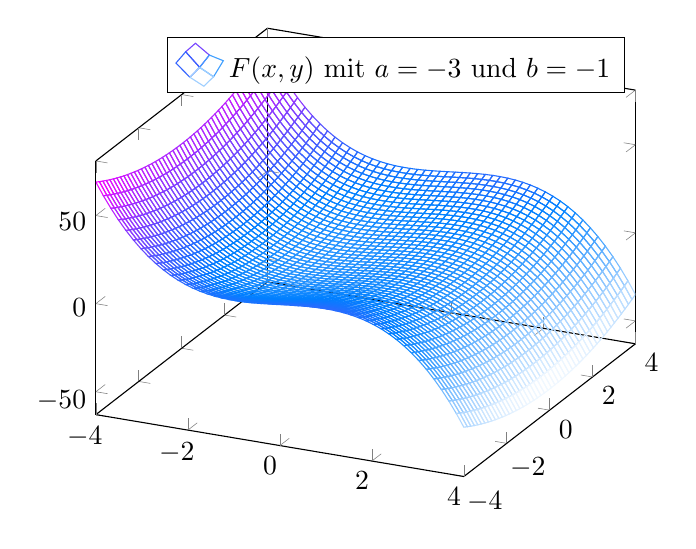
\begin{tikzpicture}
      \begin{axis}[
          % show axis
          colormap/cool,]
      \addplot3[
          mesh,
          samples=50,
          domain=-4:4,]
      {y^2 - x^3 + 3*x + 1};
      \addlegendentry{$F(x,y)$ mit $a = -3$ und $b = -1$}
      \end{axis}
    \end{tikzpicture}
  \end{center}

  Ist $M = \{(x,y) \mid F(x,y) = 0\}$ eine Teilmannigfaltigkeit?
  $$DF(x,y) = \begin{pmatrix}
    - 3x^2 - a & 2y
  \end{pmatrix} \in M(2 \times 1, \R) = grad(F)(x,y)$$
  Kritische Punkte sind $\{(x,y) \mid DF(x,y) = 0\} = \left\{\left(\pm \sqrt{\dfrac{-a}{3}},0\right)\right\}$ falls $a \leq 0$ und $\emptyset$ sonst.

  Folgt: Falls $a > 0$ oder falls $a \leq 0$ und $\left(\pm \sqrt{\dfrac{-a}{3}},0\right) \notin M$, dann ist $M$ eine Teilmannigfaltigkeit.
  Der Punkt $\left(\pm \sqrt{\dfrac{-a}{3}},0\right)$ ist $\in M$, falls $\pm \sqrt{\frac{-a}{3}}$ eine Wurzel von $x^3 + ax + b$ ist. Mit anderen Worten, falls $x^3 + ax + b$ eine doppelte Nullstelle hat.

  Beispiel: $y^2 - (x^3 - 3x + 2)$ oder $y^2 - x^3$
\end{Beispiel}

\begin{Beispiel}
  Sei $A \in M(n \times n, \R)$ symmetrisch.
  $Q: \R^n \to \R \quad Q(x) = <x, Ax> = x^T A x$
  $$M = \{x \in \R^n \mid Q(x) = 0, x \neq 0\}$$
  ist eine Quadrik.

  $$Q(x) = \sum \limits_{i,j = 1}^n a_{ij} x_i x_j$$

  $$\begin{aligned}
    \dfrac{\partial}{\partial x_k} Q(x) & = \sum \limits_{j=1}^n a_{kj} x_j + \sum \limits_{i = 1}^n a_{ik} x_i \\
    & = 2 \cdot \sum \limits_{j=1}a_kj x_j \\
    & = 2 x^T A x
  \end{aligned}$$
  Also ist $DQ(x) = 2 \cdot x^T A = grad(Q)(x)$. Folgt, dass falls $A$ invertierbar ist, so ist der einzige kritische Punkt von $Q$ der Punkt $0 \in \R^n$ und somit $M$ eine Mannigfaltigkeit der Dimension $n-1$
\end{Beispiel}

\begin{Beispiel}[Kegelschnitte]
  $$r, s \in \R, s > 0 \quad (a,b,c) \neq (0,0,0)$$
  $$K: x^2 + y^2 = sz^2$$
  $$E: ax + by + cz = r$$
  Betrachte den Schnitt $K \cap E$
  \begin{center}
    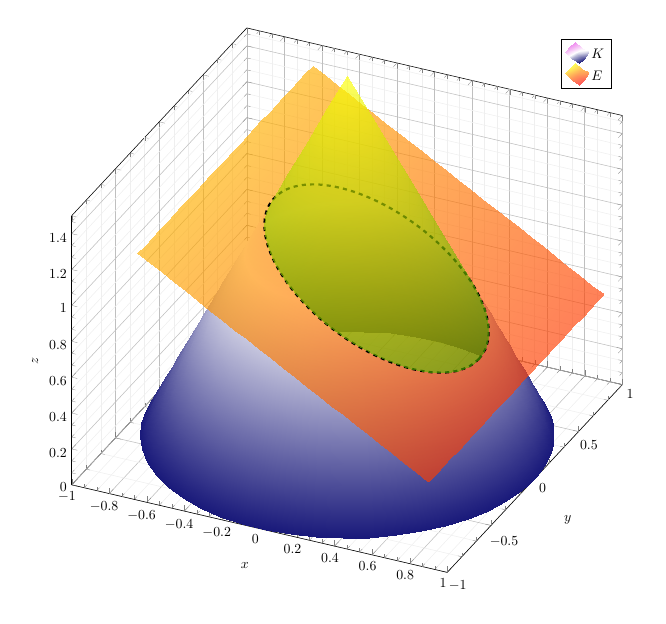
\begin{tikzpicture}[scale=0.5]
        \begin{axis}[
            axis equal image,
            grid = both,
            minor tick num = 2,
            xlabel = {$x$},
            ylabel = {$y$},
            zlabel = {$z$},
            major grid style = {draw = lightgray},
            minor grid style = {draw = lightgray!25},
            legend cell align={left},
            ymin = -1, ymax = 1,
            xmin = -1, xmax = 1,
            scale = 3,
            zmin = 0, zmax = 1.5,
            z buffer = sort,
        ]
            % bottom of the cone
            \addplot3[
                surf,
                shader = interp,
                samples = 50,
                samples y = 20,
                domain = 0:2*pi,
                domain y = 0:1,
                colormap/violet,
            ]
            (
                {cos(deg(x)) + ((sin(60) /
                (2*sin(60)-cos(60)*cos(deg(x))))*cos(deg(x))-cos(deg(x)))*y},
                {sin(deg(x)) + ((sin(60) /
                (2*sin(60)-cos(60)*cos(deg(x))))*sin(deg(x))-sin(deg(x)))*y},
                {0 + (-2*(sin(60) /
                (2*sin(60)-cos(60)*cos(deg(x))))+2-0)*y}
            );

            % plane
            \addplot3[
                surf,
                shader = interp,
                opacity = 0.65,
                domain = -0.65:0.9,
                domain y = -1:1,
                colormap/redyellow
            ]   {-cos(60)/sin(60)*x+1};

            % ellipse
            \draw[
                samples = 50,
                smooth,
                domain = 0:2*pi,
                variable = \t,
                dashed,
                ultra thick
            ]
            plot (
                {(sin(60) /
                (2*sin(60) - cos(60)*cos(deg(\t))))*cos(deg(\t))},
                {(sin(60) /
                (2*sin(60) - cos(60)*cos(deg(\t))))*sin(deg(\t))},
                {-2*(sin(60) /
                (2*sin(60) - cos(60)*cos(deg(\t))))+2}
            );

            % top of the cone
            \addplot3[
                surf,
                shader = interp,
                samples = 50,
                samples y = 5,
                domain = 0:2*pi,
                domain y = 0:1,
                opacity = 0.65,
                colormap/greenyellow,
            ]
            (
                {0 + ((sin(60) /
                (2*sin(60)-cos(60)*cos(deg(x))))*cos(deg(x))-0)*y},
                {0 + ((sin(60) /
                (2*sin(60)-cos(60)*cos(deg(x))))*sin(deg(x))-0)*y},
                {2 + (-2*(sin(60) /
                (2*sin(60)-cos(60)*cos(deg(x))))+2-2)*y}
            );

            \legend{$K$, $E$,}
        \end{axis}
    \end{tikzpicture}
  \end{center}

  Wir verwenden
  $$\begin{aligned}
    F: \R^3 & \to \R^2 \\
    F(x,y,z) & = (x^2 + y^2 -sz^2, ax + by + cz -r)
  \end{aligned}$$

  Unsere Frage, ob $K \cap E$ eine Mannigfaltigkeit ist, lässt sich zurückführen auf die Frage, ob
  $$M := \{(x,y,z) \in \R^3 \mid F(x,y,z) = 0\}$$
  eine Mannigfaltigkeit ist.

  $$DF(x,y,z) = \begin{pmatrix}
    2x & 2y & -2sz \\
    a & b & c
  \end{pmatrix}$$
  Wir wissen schon einmal $(a,b,c) \neq 0$, also hat die Matrix zumindest Rang $1$.

  $$Rang < 1 \Leftrightarrow \E \lambda \in \R : \left \{ \begin{array}{c}
    x = \lambda a \\ y = \lambda b \\ -sz = \lambda c
  \end{array}\right.$$
  Also prüfen wir:
  $$(x,y,z) = \left(\lambda a, \lambda b, -\dfrac{\lambda c}{s}\right) \in M(1 \times 3)$$
  $\lambda = 0 \quad r = 0$ oder $\lambda \neq 0 \Rightarrow r = 0$ und $E$ liegt am Kegel an. (und eine Mannigfaltigkeit, aber das kann uns der Satz des konstanten Rangs nicht sagen.)
\end{Beispiel}

\section{Tangentialräume}

\begin{Definition}[Tangentialraum]
  Es sei $M \subseteq \R^n$ eine Mannigfaltigkeit, $p \in M$. Der \textbf{Tangentialraum} von $M$ an $p$ ist
  $$T_p M = \{\gamma'(0) \mid \gamma: (-\delta,+\delta) \to M \text{ differenzierbar }, \gamma(0) = p, \delta > 0 \} \subseteq \R^n$$
  Elemente von $T_p M$ nennt man \textbf{Tangentialvektoren} und
  $$T M = \{(p,v) \mid p \in M, v \in T_p M\}\subseteq M \times \R^n \subseteq \R^n \times \R^n$$
  nennt man \textbf{Tangentialbündel} von $M$.
\end{Definition}

\begin{Bemerkung}
  $$0 \in T_p M$$
  betrachte hierfür einfach den Pfad $\kappa = p$ (konstant).

  Später werden wir sogar sehen, dass $T_p M$ ein Untervektorraum von $\R^n$ ist:
  $$v \in T_p M \Rightarrow \lambda \cdot v \in T_p M \A \lambda \in \R$$

  Wir können allerdings noch nicht sagen, ob gilt
  $$v_1, v_2\in T_p M \Rightarrow v_1 + v_2 \in T_p M$$
\end{Bemerkung}

\begin{Bemerkung}
  $$\begin{aligned}
    \pi: TM & \to M \\
    (p,v) & \mapsto p
  \end{aligned}$$
  ist die kanonische Projektion, und wir haben eine umgekehrte Abbildung:
  $$\begin{aligned}
    0_M: M & \to TM \\
    p & \mapsto (P,0)
  \end{aligned}$$
  die wir Nullschnitt nennen.
\end{Bemerkung}

\begin{Definition}[Vektorfeld]
  Eine Abbildung $s: M \to T M$ mit $\pi \circ s = id_M$ heißt \textbf{Schnitt} oder auch \textbf{Vektorfeld} von $M$.
  $$\begin{aligned}
    s: M & \to TM \\
    p & \mapsto (p,v)
  \end{aligned}$$
\end{Definition}

Nachfolgend verwenden wir folgende Notation.
$$\R^k = \R^k \times \{0\} \subseteq \R^n$$

\begin{Theorem}
  Sei $M \subseteq \R^n$ eine Teilmannigfaltigkeit, $U \subseteq \R^n$, $V \subseteq \R^n$ offen. Sei $\psi: V \to U$ ein Diffeomorphismus mit $\psi(\R^k \cap V) = U \cap M$. (also wäre $\psi^{-1}$ eine Karte).

  Dann ist die Abbildung
  $$\begin{aligned}
    T \psi: (V \cap \R^k) \times \R^k & \to T(U \cap M) \\
    T\psi(y,h) & = (\psi(y),D\psi(y)(h))
  \end{aligned}$$
  wohldefiniert und eine Bijektion. Insbesondere gilt für $p = \psi(y)$
  $$T_p M = Im(D\psi(y) : \R^k \to \R^n)$$
  Da $D\psi$ eine lineare Abbildung ist, ist $T_p M$ insbesondere ein linearer Unterraum der Dimension $k$ von $\R^n$.
\end{Theorem}

\begin{Beweis}
  Da $V \cap \R^k$ offen in $\R^k$ ist (relativ offen), existiert zu jedem $y \in V \cap \R^k$ ein $\delta >0$ so, dass
  $$\begin{aligned}
    \gamma: (-\delta, \delta) & \to V \cap \R^k \\
    t & \mapsto y + th
  \end{aligned}$$
  wohldefiniert ist. Es gilt dann: $\gamma(0) = y$ und $\gamma'(0) = h$.

  Damit ist $\psi \circ \gamma$ ein Pfad im $M$ mit $(\psi \circ \gamma)(0) = \psi(y)$ und
  $$\begin{aligned}
    (\psi \circ \gamma)'(0) & = D \psi(\gamma(0))\cdot \gamma'(0)\\
    & = D\psi(y)(h) \in T_{\psi(y)} M
  \end{aligned}$$
  $$\Rightarrow T \psi \text{ ist wohldefiniert}$$
  \begin{itemize}
    \item $T\psi$ injektiv: Weil $\psi$ injektiv ist und $D\psi(y)$ injektiv ist für alle $y \in \R^k$.
    \item $T \psi$ surjektiv: Sei $p = \psi(y) \in M$ und $\gamma: (-\delta,\delta) \to M$ mit $\gamma(0) = p$ und $v = \gamma'(0) \in T_p M$.

      Betrachte $\psi^{-1} \circ \gamma$, einen Pfad in $\R^k \cap V$.
      $$\begin{aligned}
        h:= (\psi^{-1} \circ \gamma)'(0) & = D \psi^{-1}(p)(v) \\
        & = (D \psi(y))^{-1}(v)
      \end{aligned}$$
      Also gilt: $D\psi(y)(h) = v$ und es folgt $T\psi(y,h) = (p,v)$. Also ist $\psi$ surjektiv.
  \end{itemize}
  Nochmal eine zusammenfassende Beweisskizze: Wir können die Teilmannigfaltigkeit in eine lineare Untermenge des $\R^k$ überführen, und dann dort unsere Aussagen zeigen und sie anschließend wieder zurück auf $M$ anzuwenden. Das ist möglich weil $\psi$ als Diffeomorphismus bijektiv ist.
  \incfig{projektion}
\end{Beweis}

\begin{Theorem}
  Sei $U \subseteq \R^n$, $F: U \to \R^m$ glatt und $M:=F^{-1}(0)$. Angenommen $DF(p): \R^n \to \R^m$ sei surjektiv für alle $p \in M$ (also ist $M$ eine Mannigfaltigkeit der Dimension $k = n - m$). Dann gilt
  $$T_p M = \ker(DF(p): \R^n \to \R^m)$$
\end{Theorem}

\begin{Beweis}
  $T_p M$ und $\ker(DF(p)$n sind $k$-dimensionale lineare Unterräume des $\R^n$. Es genügt also Inklusion des Einen im Anderen zu zeigen.

  Wir schauen uns $T_p M \subseteq \ker(DF(p)$ an: Sei $\gamma:(-\delta,\delta) \to M$ mit $\gamma(0) = p$.
  $$DF(p)(\gamma'(0)) = \underbrace{(F \circ \gamma)'}_{\equiv 0}(0) = 0$$
  Also $\gamma'(0) \in \ker(DF(p)$
\end{Beweis}

\begin{Beispiel}
  $$U = \R^3 \qquad \left\{\begin{aligned}
    F: U & \to \R \\
    F(x,yz) & = (2x^2 + y^2 + z^2 - 1)^3 - \frac{1}{10}x^2 z^3 - y^2z^3
  \end{aligned}\right.$$
  Seien $M = F^{-1}(0)$ und $p = (0,1,1) \in M$. Dann ist
  $$DF(x,y,z) = \begin{pmatrix}
      12x(2x^2 + y^2 + z^2 -1)^2 - \frac{1}{5}xz^3 \\
      6y(2x^2 + y^2 + z^2 -1)^2 - 2 yz^3 \\
      6z(2x^2 + y^2 +z^2 -1)^2 - \frac{3}{10}x^2z^2 - 3y^2z^2
    \end{pmatrix} \Rightarrow DF(p) = \begin{pmatrix}
      0 \\ 4 \\ 3
    \end{pmatrix}$$
  Also gilt: $\ker(DF(p)) = \left<\begin{pmatrix}
    1 \\ 0 \\ 0
  \end{pmatrix}, \begin{pmatrix}
    0 \\ -3 \\ 4
  \end{pmatrix} \right>$ und man kann zeichnen:

  \begin{center}
  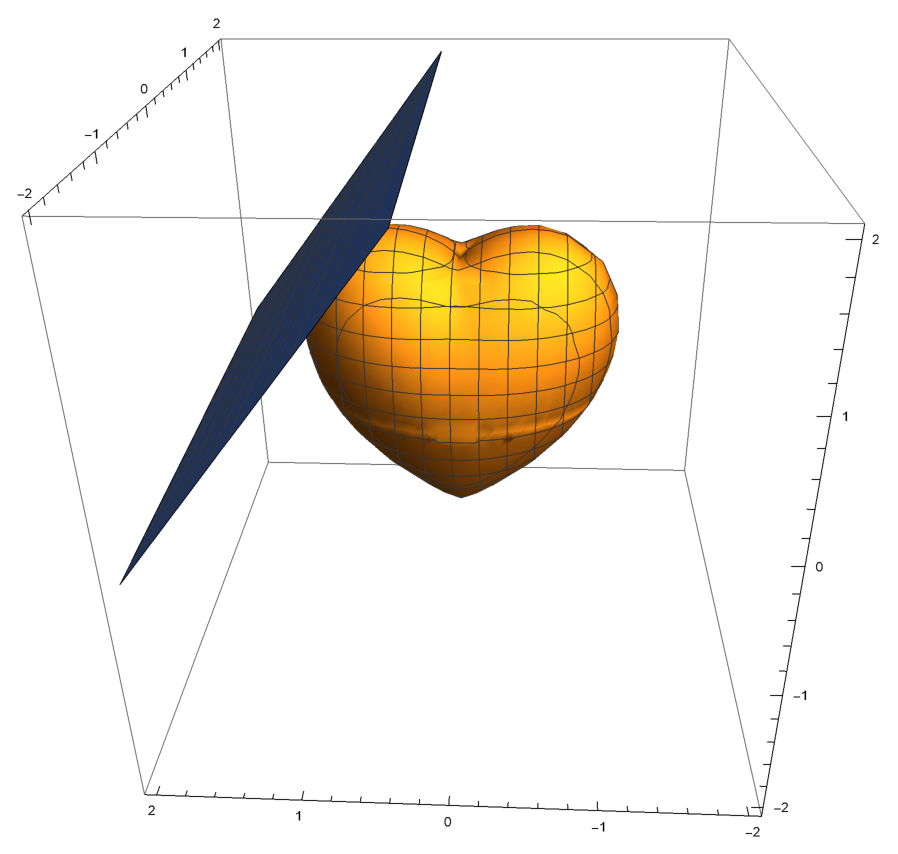
\includegraphics[scale = 0.5]{./img/tangentialraum_beispiel}
    % \begin{tikzpicture}
    %   \begin{axis}[
    %       % show axis
    %       colormap/cool,]
    %   %\addplot3[
    %   %    mesh,
    %   %    samples=50,
    %   %    domain=-2:2,]
    %   %{(2*x^2 + y^2 + z^2 - 1)^3 - (1/10) * x^2 * z^3 - y^2 * z^3 == 0};
    %   %\addlegendentry{$F = 0$}
    %   \addplot3[
    %       mesh,
    %       samples=50,
    %       domain=-2:2,]
    %   {4*y + 3*z == 7};
    %   \addlegendentry{Tangentialebene}
    %   \end{axis}
    % \end{tikzpicture}
  \end{center}
  Ist das nicht süß?
\end{Beispiel}

\begin{Beispiel}
  $$M = \{(x,y,z) \in \R^3 \mid \underbrace{x^2 + y^2 = z}_{A} ,\quad \underbrace{y+y+z = 1}_{B}\}$$
  \begin{itemize}
    \item[$A)$] Die Parabel $x^2 = z$ um die $z$-Achse rotiert.
    \item[$B)$] Ebene durch $\left(\begin{smallmatrix} 1 \\ 0 \\ 0 \end{smallmatrix}\right)$, $\left(\begin{smallmatrix} 0 \\ 1 \\ 0 \end{smallmatrix}\right)$ und $\left(\begin{smallmatrix} 0 \\ 0 \\ 1 \end{smallmatrix}\right)$.
  \end{itemize}
  Betrachte
  $$\begin{aligned}
    F: \R^3 & \to \R^2 \\
    F(x,y,z) & = \begin{pmatrix}
      x^2 + y^2 - z\\
      y + y +z -1
    \end{pmatrix}
  \end{aligned}$$
  Also ist $M = F^{-1}(0)$
  $$DF(x,y,z) = \begin{pmatrix}
    2x & 2y & -1 \\
    1 & 1 & 1
  \end{pmatrix}$$
  $Rang(DF(x,y,z)) < 2 \Leftrightarrow x = y = -\dfrac{1}{2}$ und $z$ beliebig. Aber dieser kritische Punkt $\notin M$ für alle $z \in \R$.

  Also ist $M$ eine Mannigfaltigkeit und
  $$\begin{aligned}
    T_p M & = \ker( DF(p)) \A p \in M \\
    & p := \left(\frac{1}{\sqrt{2}},-\frac{1}{\sqrt{2}},1 \right) \in M \\
    DF(p) & = \begin{pmatrix}
      \sqrt{2} & - \sqrt{2} & -1 \\
      1  & 1 & 1
    \end{pmatrix} \\
    & = \left< \begin{pmatrix}
      \sqrt{2} + 1 \\
      -\sqrt{-2} - 1 \\
      0
    \end{pmatrix}\right>
  \end{aligned}$$
\end{Beispiel}

\begin{Beispiel}
  $$SL_2 = \left \{ A = \left(\begin{smallmatrix}
    a & b\\c & d
  \end{smallmatrix} \right) \Big | det(A) = ad - bc = 1 \right \} \subseteq \R^4$$
  also anders dargestellt
  $$M = \{x \in \R^4 \mid F(x) = x_1x_4 - x_2x_3 -1 = 0\} \subseteq \R^4$$
  Wie sonst auch berechnen wir also

  Sei $p = \left(\begin{smallmatrix}
    1 & 0 \\ 0 & 1
  \end{smallmatrix}\right) \equiv (1,0,0,1)$, die Einheitsmatrix. Nun berechnen wir
  $$DF(x) = (x_4, -x_3, -x_2,x_1)$$
  und es gilt
  $$DF(x) = 0 \Leftrightarrow x = 0 \quad 0 \neq M$$
  also ist $M$ eine Mannigfaltigkeit.
  $$\begin{aligned}
    T_p M = \ker(DF(p)) & = \ker((1 \, 0 \, 0 \, 1))\\
    & = \left<\left(\begin{smallmatrix}
      0 \\ 1 \\ 0 \\ 0
    \end{smallmatrix}\right),\left(\begin{smallmatrix}
      0 \\ 0 \\ 1 \\ 0
    \end{smallmatrix}\right),\left(\begin{smallmatrix}
      1 \\ 0 \\ 0 \\ -1
    \end{smallmatrix}\right)\right>
  \end{aligned}$$
  In der Matrizensprache ergibt das
  $$T_{id} SL_2 = \left< \left(\begin{smallmatrix}
    0 & 1 \\ 0 & 0
  \end{smallmatrix}\right), \left(\begin{smallmatrix}
    0 & 0 \\ 1 & 0
  \end{smallmatrix}\right), \left(\begin{smallmatrix}
    0 & 0 \\ 0 & 1
  \end{smallmatrix}\right) \right> = \{A \in M(2\times2,\R) \mid tr(A) = 0\}$$
\end{Beispiel}


\section{Extremwertprobleme}

Sei $M \subseteq U \subseteq \R^n$ offen und $f: U \to \R$ differenzierbar. Versuchen wir das Maximum von $f|_M$ zu finden.

Beispiel: $M = \mathcal{S}^{n-1} \subseteq \R^n$ und $f: \R^n \to \R$ Polynomial.

\begin{Definition}[Normalenraum]
  Sei $M \subseteq \R^n$ eine Mannigfaltigkeit der Dimension $k$. Sei $p \in M$. Wir nennen
  $$N_p M = (t_p M)^\perp = \{w \in \R^n \mid <w,v> = 0 \A v \in T_pM\}$$
  den $(n-k)$-dimensionalen \textbf{Normalenraum} von $M$ in $p$.

  Wir nennen $w \in N_p M$ einen \textbf{Normalenvektor} von $M$ bei $p$.

  Das \textbf{Normalenbündel} von $M$ ist
  $$\{(p,w) \mid p \in M \text{ und } w \in N_pM\}$$
\end{Definition}

\begin{Bemerkung}
  Auch hier existiert eine kanonische Projektion
  $$\begin{aligned}
    \pi : NM & \to M \\
    (p,w) & \mapsto p
  \end{aligned}$$
\end{Bemerkung}

\begin{Bemerkung}
  Ist $M$ als Niveaumenge gegeben, etwa $M := F^{-1}(0)$, $F: U \to \R^n$ so definiert, dass $0$ ein regulärer Wert von $F$ ist.

  Sei $p$ ein Element von $M$, dann ist
  $$DF(p): \R^n \to \R^m$$
  surjektiv und $T_pM = \ker DF(p)$.

  Konkret ist
  $$DF(p) = \left(\dfrac{\partial}{\partial x_j} F_i(p)\right)_{i,j} \in M(n \times m, \R)$$
  und $v \in T_p M \Leftrightarrow DF(p)(v) = 0 \Leftrightarrow A \cdot v = 0 \Leftrightarrow <grad \, F_i(p),v> = 0 < m \A i $.

  Folgt $grad \, F_i(p) \in N_p M$

  Da $DF(p)$ Rang $m$ hat, bilden die Vektoren
  $$\{grad \, F_i(p) \mid i = 1,2,...,m\}$$
  eine Basis von $N_p M$.
\end{Bemerkung}

\begin{Beispiel}
  $$\begin{aligned}
    F: \R^3 & \to \R \\
    F(x,y,z) & = e^{xyz} + x + y^2 + z^3 - 1
  \end{aligned}$$
  Sei $M = F^{-1}(0)$ und $p = (0,0,0)\in M$.
  $$DF(p) = \begin{pmatrix}
    1 & 0 & 0
  \end{pmatrix}$$
  und man erkennt
  $$N_p M = \left< \left( \begin{smallmatrix}
    1 \\ 0 \\ 0
  \end{smallmatrix}\right)\right> \quad T_p M = \left< \left( \begin{smallmatrix}
    0 \\ 1 \\ 0
  \end{smallmatrix}\right), \left( \begin{smallmatrix}
    0 \\ 0 \\ 1
  \end{smallmatrix}\right)\right>$$
\end{Beispiel}

\begin{Beispiel}
  $$F(x,y,z) = \begin{pmatrix}
    x^2 + y^2 - z \\
    x + y + z - 1
  \end{pmatrix}$$
  $F^{-1} = 0$ und $p = (x_0, y_0, z_0) \in M$. Also:
  $$DF(p) = \begin{pmatrix}
    2x_0 & 2y_0 & -1 \\
    1 & 1 & 1
  \end{pmatrix}$$
  und
  $$N_p M = \left< \left( \begin{smallmatrix}
    2x_0 \\ 2y_0 \\ -1
  \end{smallmatrix}\right), \left( \begin{smallmatrix}
    1 \\ 1 \\ 1
  \end{smallmatrix}\right)\right>$$
\end{Beispiel}

\begin{Theorem}
  Sei $M \subseteq U \subseteq \R^n$ eine Mannigfaltigkeit mit $U$ offen und $f: U \to \R$ stetig differenzierbar. Sei $p \in M$. Falls $p$ ein lokales Extremum von $f|_M$ ist, so gilt
  $$grad \, f(p) \in N_p M$$
\end{Theorem}

\begin{Beweis}
  Sei $v \in T_p M$ beliebig. Zu zeigen: $< grad \, f(p), v> = 0$.

  Sei $\gamma: (-1,1) \to M$ ein Pfad, also $\gamma(0) = p$ und $\gamma'(0) = v$. Dann ist $0$ ein lokales Extremum von $f \circ \gamma: (-1,1) \to \R$
  $$\begin{aligned}
    0 = (f \circ \gamma)' (0) & = Df(\gamma(0))(\gamma'(0)) \\
    & = Df(p)(v) \\
    & = < grad \, f(p),v>
  \end{aligned}$$
\end{Beweis}

\begin{Bemerkung}[Strategie]
  Hiermit können wir sehr oft loakle Extrema von $f: U \to \R$ auf einer Teilmenge $M$ finden.
  \begin{enumerate}
    \item Berechne $N_p M$ für alle (fast alle) $p \in M$
    \item Finde alle $p \in M$ mit $grad \, f(p) \in N_p M$ (LGS). Diese Punkte $p$ sind Kandidaten für lokale Extrema.
    \item Alle Punkte $p \in M$, an denen $N_p M$ nicht definiert ist, oder $f$ nicht differenzierbar ist, sind auch Kandidaten.
    \item Entscheide ad-hoc, ob und welche Kandidaten Extrema sind.
  \end{enumerate}
\end{Bemerkung}

\begin{Beispiel}
  $$K = \{(x,y) \in \R^2 \mid |x| \leq 1, |y| \leq 1, x^2 = y^3\}$$
  also ist
  $$M = K \backslash \{(0,0), (1,1), (-1,1)\}$$ eine Mannigfaltigkeit, gegeben durch die Nullstellen von
  $$\begin{aligned}
    (-1,1)^2 \backslash \{0\} & \to \R \\
    (x,y) & \mapsto y^3 - x^2
  \end{aligned}$$

  \begin{center}
    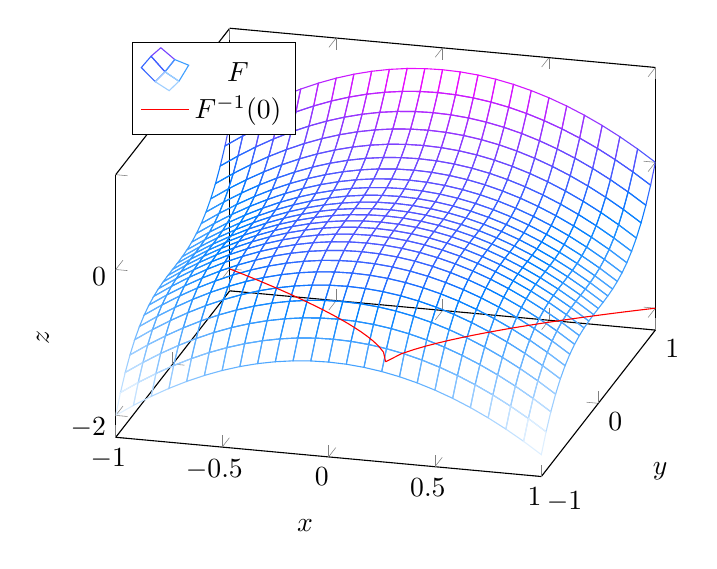
\begin{tikzpicture}
      \begin{axis}[
        view={15}{30},
        domain=-1:1,
        domain y=-1:1,
        xlabel={$x$},
        ylabel={$y$},
        zlabel={$z$},
        colormap/cool,
        legend pos=north west,
      ]
        \addplot3[mesh,samples=25]{y^3 - x^2};
        \addlegendentry{$F$}
        \addplot[red,domain=-1:0] {(-x)^(2/3)};
        \addlegendentry{$F^{-1}(0)$}
        \addplot[red,domain=0:1] {x^(2/3)};
      \end{axis}
    \end{tikzpicture}
  \end{center}

  Finde alle lokalen Extrema der Funktion $f(x,y) = 4y - 3x$ auf $K$.

  Wir wenden also jetzt unsere Strategie an:
  \begin{enumerate}
    \item Für $p = (x_0,y_0)$ gilt $DF(p) = \begin{pmatrix}
        -2x_0 & 3 y_0^2
      \end{pmatrix}$.

      Für $p \in M$ spannt $\left( \begin{smallmatrix} -2 x_0 \\ 3y_0^2 \end{smallmatrix}\right)$ den Raum $N_p M$ auf.
    \item Es gilt $grad \, f(p) = \begin{pmatrix}
        -3 & 4
      \end{pmatrix}$
  \end{enumerate}

  Um Punkte $p$ mit $grad \, f(p) \in N_p M$ zu finden, lösen wir
  $$\begin{pmatrix}
      -3 \\ 4
    \end{pmatrix} = \lambda \cdot \begin{pmatrix}
        -2x_0 \\ 3 y_0^2
    \end{pmatrix}$$
    Wir erhalten das Gleichungssystem
    $$\left\{\begin{aligned}
      3 & = -2 \lambda x_0 \\
      4 & = 3 \lambda y_0 \\
      x_0^2 = y_0^3
    \end{aligned}\right.  \left\} \dfrac{4}{3} = \dfrac{3 y_0^2}{2 x_0} \right. \Rightarrow x_0 = \dfrac{9}{8} y_0^2$$
    Jetzt haben wir
    $$0 = x_0^2 - y_0^3 = \left(\dfrac{9}{8} y_0^2\right)^2 - y_0^3 =  \left(\dfrac{9^2}{8^2} y_0 - 1\right) y_0^3$$
    $$\Rightarrow y_0 = \dfrac{9^2}{8^2} \quad x_0 = \dfrac{9^3}{8^3} \quad p=\left(\dfrac{9^2}{8^2},\dfrac{9^3}{8^3}\right)$$
  \item Für unsere 4 Kandidaten rechnen wir aus:
    \begin{itemize}
      \item $f(0,0) = 0$ also ein globales Minimum
      \item $f(1,1) = 1$ also ein lokales Minimum
      \item $f(-1,1) = 7$ also ein globales Maximum
      \item $f(p) = 4 \cdot \dfrac{9^3}{8^3} - 3 \cdot \dfrac{9^2}{8^2} \sim 1,053$ also ein lokales Maximum
    \end{itemize}
\end{Beispiel}

\begin{Definition}[Lagrange Multiplikatoren]
  Sei $U \subseteq \R^n$ offen, $F: U \to \R^n$ mit $0$ als regulärem wert und $M = F^{-1}(0)$ eine Mannigfaltigkeit der Dimension $k = n-m$. Sei $\varphi: U \to \R$ von Klasse $\mathcal{C}^1$. Die zu $f, F$ assozieerte \textbf{Lagrange-Funktion} ist
  $$\begin{aligned}
    L:U \times \R^m & \to \R \\
    L(x,\lambda) & = f(x) - <\lambda, F(x)>
  \end{aligned}$$
  $\lambda = (\lambda_1,...,\lambda_m)$ sind die \textbf{Lagrange-Multiplikatoren}.
\end{Definition}

\begin{Theorem}
  In der obigen Situation gilt: Ist $p \in U$ ein lokales Extremum von $f$ auf $M$, dann existiert $\lambda \in \R^n$ mit
  \begin{enumerate}
    \item $\dfrac{\partial}{\partial x_i} L(p,\lambda) = 0 \quad i =1,2,...,n$
    \item $\dfrac{\partial}{\partial \lambda_i} L(p,\lambda) = 0 \quad i =1,2,...,n$
  \end{enumerate}
  oder kompakt
  $$DL(p,\lambda) = 0$$
\end{Theorem}

\begin{Beweis}
  $$\begin{aligned}
    \dfrac{\partial}{\partial \lambda_i} L(p,\lambda) & = \dfrac{\partial}{\partial \lambda_i} \left(f(x) - \sum \limits_{l=1}^m\lambda_lF_l(x) \right) \\
    & = -F_i(p) \\
    2) \, \Leftrightarrow F(p) & = 0
  \end{aligned}$$
  $$0 = \dfrac{\partial}{\partial x_i}\left(f(p) - \sum \limits_{l=1}^m \lambda_l F_l(p)\right) = \dfrac{\partial}{\partial x_i} f(p) - \sum \limits_{l=1}^m \lambda \dfrac{\partial}{\partial x_i} F(p)$$
  $$grad \, f(p) = \sum \limits_{l=1}^m \lambda_l \cdot grad \, F_l(p)$$
  $$\Leftrightarrow grad \, f(p) \in N_p M$$
\end{Beweis}

\subsection{Satz von Lagrange}

Gegeben sind $U \subseteq \R^n$ offen, $F: U \to \R^m$ mimt $0$ als regulärem Wert. Wir definieren $M := F^{-1}(0)$. Sei $f: U \to \R$ und wir wollen die Extrema von $f\mid_M$ finden.

\begin{Theorem}[Methode von Lagrange]
  Ist $p \in M$ mit $grad \, f(p) \in N_p M$, dann ist $p$ ein Kandidat für ein lokales Extremum von $f |_M$.
\end{Theorem}

\begin{Beweis}
  $$grad \, f(p) \in N_p M \Leftrightarrow grad \, f(p) = \sum \limits_{i=1}^m \lambda_i \cdot grad \, F_i(p)$$
  $\lambda_i \in \R$ sind die Lagrange-Multiplikatoren
\end{Beweis}

\begin{Beispiel}
  Finde das Maximum von
  $$f(x,y,z) = e^{xyz}$$
  auf
  $$M = \{(x,y,z) \in \R^3 \mid x^2+y^2 = z, x+y+z = 1\} \subseteq \R^3$$
  Wir definieren
  $$\begin{aligned}
    F : \R^3 & \to \R^2 \\
    F(x,y,z) & = \begin{pmatrix}
      x^2 + y^2 - z \\ x + y + z - 1
    \end{pmatrix}
  \end{aligned}$$
  und man erkennt, dass $M = F^{-1}(0)$.

  Da die Ableitung von $F$ immer surjektiv ist, für alle Werte $p \in M$, ist $M$ eine Teilmannigfaltigkeit von $\R^3$.

  $$grad \, f(x,y,z) = \begin{pmatrix}
    yz \cdot e^{xyz} & xz \cdot e^{xyz} & xy \cdot e^{xyz}
  \end{pmatrix}$$
  und
  $$DF(x,y,z) = \begin{pmatrix}
    2x & 2y & -1 \\
    1 & 1 & 1
  \end{pmatrix}$$
  Also ist unser Gleichungssystem:
  $$(yz,xz,xy) \cdot e^{xyz} = \lambda(2x,2y,-1) + \mu(1,1,1)$$
  $$\Leftrightarrow \left \{ \begin{aligned}
      x^2 + y^2 & = z \\
      x + y + z & = 1 \\
      yz \cdot e^{xyz} & = 2 \lambda x + \mu \\
      xz \cdot e^{xyz} & = 2 \lambda y + \mu \\
      xy \cdot e^{xyz} & = - \lambda + \mu
    \end{aligned}\right.$$
  Es genügt dann (hem hem), das Gleichungssystem zu lösen.
\end{Beispiel}

\begin{Beispiel}
  Finde $\left(\begin{smallmatrix}
    a & b \\ c & d
  \end{smallmatrix}\right) \in SL_2(\R)$ so dass die Frobemius-Norm $\sqrt{a^2 + b^2 + c^2 + d^2}$ minimal ist.

  Betrachte $M: \{(x_1,...,x_4) \in \R^4 \mid \underbrace{x_1x_4 - x_2x_3 - 1}_{F(x)} = 0\}$

  und $f(x) = x_1^2 + x_2^2 + x_3^2 + x_4^2 = ||x||_F^2$.
  $$grad \, f(x) = \begin{pmatrix}
    2x_1 & 2x_2 & 2x_3 & 2x_4
  \end{pmatrix} = 2x$$
  $$grad \, F(x) = \begin{pmatrix}
    x_4 & -x_3 & -x_2 & x_1
  \end{pmatrix}$$
  Wir erhalten das folgende Gleichungssystem.
  $$\left\{\begin{aligned}
    x_1x_4 - x_2x_3 - 1 & = 0 \\
    2x_1 & = \lambda \cdot x_4 \\
    2x_2 & = -\lambda \cdot x_3 \\
    2x_3 & = -\lambda \cdot x_2 \\
    2x_4 & = \lambda \cdot x_1
  \end{aligned}\right.$$
  Man erkennt, dass $\lambda^2 = 1$ also $\lambda = \pm 1$.
  $$\lambda = 1 \Rightarrow x = (t,s,-s,t) \rightsquigarrow \left(\begin{smallmatrix}
    a & b \\ -b & a
  \end{smallmatrix}\right)$$
  $$\lambda = 1 \Rightarrow x = (t,s,s,-t) \rightsquigarrow \left(\begin{smallmatrix}
    a & b \\ b & -a
  \end{smallmatrix}\right) \notin M$$
  Wir betrachten wieder die Determinantenvoraussetzung
  $$F(x) = F(t,s,-s,t) = t^2 +s^2 - 1 = 0$$
  $\Rightarrow$ ist $x \in M$ ein lokales Extremum von $f$, so gilt
  $$x = (t,s,-s,t) : t^2 + s^2 = 1 \text{ also } t = \cos(\varphi), s = \sin(\varphi)$$
  $$f(x) = t^2 + s^2 + s^2 +t^2 = 2$$
  Also ist die Lösung:
  $$\min\{\sqrt{a^2 + b^2 +c^2 +d^2}\} = \sqrt{2}$$
  Es wird angenommen von Matrizen der Form $\left(\begin{smallmatrix}
    \cos(\varphi) & \sin(\varphi) \\
    -\sin(\varphi) & \cos(\varphi)
  \end{smallmatrix}\right)$, den orthogonalen $2 \times 2$ Matrizen.
\end{Beispiel}

\begin{Beispiel}
  2 disjunkte Mengen
  $$M_1 = \{(x,y,z) \in \R^3 \mid x^2 + 3y^2 +3z^2 = 1\}$$
  $$M_2 = \{(x,y,z) \in \R^3 \mid (x - 5)^2 + (y - 5)^2 + (z - 5)^2 = 1\}$$
  Wir suchen die Punkte $p_1$ und $p_2$ respektive in $M_1$ und $M_2$ so, dass die Distanz minimal wird.

  Wir betrachten $M_1 \times M_2 \subseteq \R^3 \times \R^3 = \R^6$ und die Funktion $f: \R^6 \to \R$ durch $f(x_1,y_1,z_1,x_2,y_2,z_2) = (x_1-x_2)^2 + (y_1 - y_2)^2 + (z_1-z_2)^2$.

  $M_1 \times M_2$ ist die Nullstellenmenge der Funktion
  $$\begin{aligned}
    F: \R^6 & \to \R^2 \\
    (x_1,y_1,z_1,x_2,y_2,z_2) & \mapsto \begin{pmatrix}
      x_1^2 + 3y_1^2 + 3 z_1^2 - 1 \\ (x_2 - 5)^2 + (y_2 - 5)^2 + (z_2 - 5)^2 -1
    \end{pmatrix}
  \end{aligned}$$
  Wir wollen das Minimum von $f |_M$ finden
  $$\begin{aligned}
    grad \, f(x_1,...z_2) & = 2 \begin{pmatrix}
    x_1 - x_2 & y_1 - y_2 & z_1 - z_2 & -(x_1 - x_2) & -(y_1 - y_2) & -(z_1 - z_2)
  \end{pmatrix}\\
  & \in M(1 \times 6, \R)
  \end{aligned}$$
  $$DF(x_1,...z_2) = \begin{pmatrix}
    2x_1 & 6y_1 & 6z_1 & 0 & 0 & 0 \\
    0 & 0 & 0 & 2(x_2 - 5) & 2(y_2 - 5) & 2(z_2 - 5)
  \end{pmatrix}$$
  Ergibt folgendes Gleichungssystem
  $$\left\{\begin{aligned}
    x_1^2 + 3y_1^2 + 3z_1^2 & = 1 \\
    (x_2 - 5)^2 + (y_2 - 5)^2 + (z_2 - 5)^2 & = 1 \\
    2(x_1 - x_2) & = 2 \lambda_1 x_1 + \lambda_2 \cdot 0 \\
    2(y_1 - y_2) & = 6 \lambda_1 y_1 + \lambda_2 \cdot 0 \\
    2(z_1 - z_2) & = 6 \lambda_1 z_1 + \lambda_2 \cdot 0 \\
    -2(x_1 - x_2) & = \lambda_1 0 + 2 \lambda_2 (x_2 -5) \\
    -2(y_1 - y_2) & = \lambda_1 0 + 2 \lambda_2 (y_2 -5) \\
    -2(z_1 - z_2) & = \lambda_1 0 + 2 \lambda_2 (z_2 -5)
  \end{aligned}\right.$$
  Aus geometrischen Überlegungen wissen wir, dass wir genau eine Lösung erhalten. Um das anfängliche Problem zu lösen müssen wir dann noch $d(p_1,p_2)$ berechnen mit $p_1 = (x_1,y_1,z_1)$ und $p_2 = (x_2,y_2,z_2)$.
\end{Beispiel}

\end{document}
